\documentclass[a4paper,12pt]{report}
\usepackage[utf8]{inputenc}
\usepackage{graphicx}
\usepackage[margin=1in]{geometry}
\usepackage{setspace}
\usepackage{amsmath}
\usepackage{caption}
\usepackage{subcaption}
%\usepackage{titlesec}


\begin{document}
\setcounter{chapter}{2}
\chapter{Creating a curved geomtery in Open Foam}
\flushleft In this chapter we will learn how to create a 2-D geometry for a flow over a cylinder. As it is an axis-symmetric geometry, we will consider the cylinder as a semi-circle and a rectangular domain around it. For meshing this geometry you should divide the domain into small hexahedral blocks. In this particular problem we have body fitted grid, as shown in Fig \ref{frontface} and Fig \ref{backface}{$:$}

\begin{figure}[ht]  
\begin{center}  
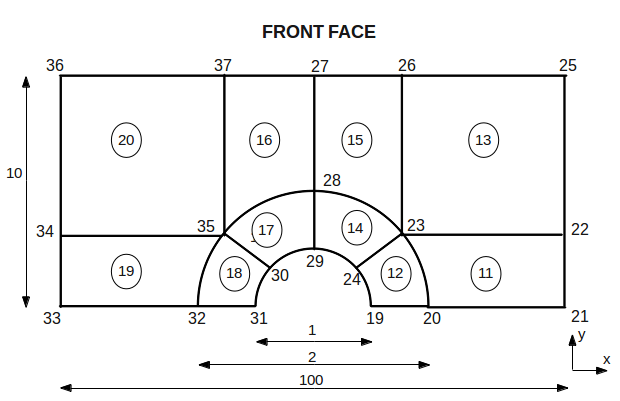
\includegraphics[scale=0.6]{frontface.png}
\caption{Geomtery points in the front face for 2-D flow over a cylinder}
\label{frontface}
\end{center}  
\end{figure}

\begin{figure}[ht]  
\begin{center}  
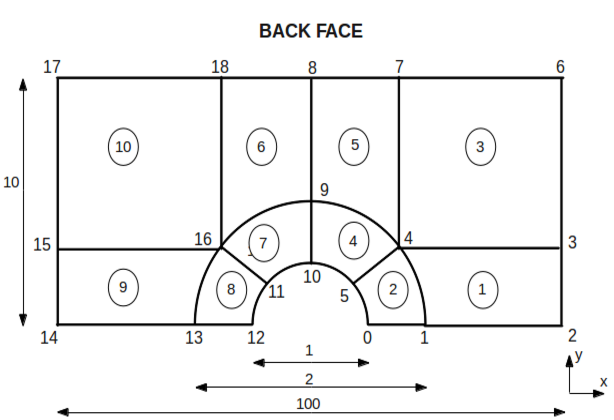
\includegraphics[scale=0.6]{backface.png}
\caption{Geomtery points in the back face for 2-D flow over a cylinder}
\label{backface}
\end{center}  
\end{figure}

\flushleft Now, as mentioned in the previous chapter create a new blockMeshDict file and open it. In this geometry file  copy the initial few lines  till “convertToMeters” from previous lid-driven cavity problem “blockMeshDict” file and paste it. Here we will keep “convertToMeters” as 1 as we have given the geometry in meters. After this write down the coordinates of the vertices of the geometry in a similar fashion as given in the previous chapter. 
\flushleft For this particular problem we have used cosine and sine function to calculate the vertices on the curved edges as shown below{$:$}

\begin{figure}[ht]  
\begin{center}  
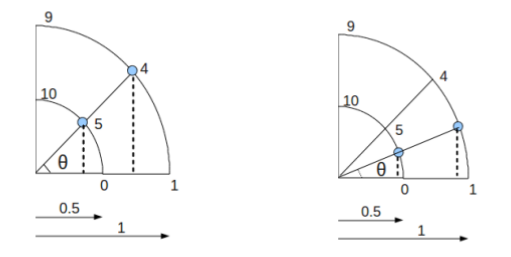
\includegraphics[scale=0.6]{angle.png}
\caption{Geomtery points for 2-D flow over a curved body}
\label{angle}
\end{center}  
\end{figure}

\flushleft where angle {$\theta$}  is calculated as{$:$}
\flushleft sin({$\theta$}) = perpendicular/hypotenuse
\flushleft cos({$\theta$}) = base/hypotenuse
\flushleft Note that you should be very careful about the order of the vertex coordinates. It should start from 0 and be continued as 1,2,3.., as shown below{$:$}
\flushleft vertices
\flushleft(
\flushleft  (0.5 0 0)	//0
\flushleft  (1 0 0)	//1
\flushleft.
\flushleft.
\flushleft.
\flushleft.
\flushleft);
\flushleft After this enter the details within blocks in a similar manner as shown in the previous chapter. Here in this problem, we have divided the geometry domain into ten small hexahedral blocks having structured body fitted grid points, as shown in fig \ref{blocks}. For further details on how to create blocks you may refer to chapter 2.

\begin{figure}[ht]  
\begin{center}  
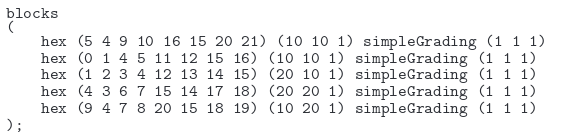
\includegraphics[scale=0.6]{blocks.png}
\caption{Block details for the blockMeshDict file}
\label{blocks}
\end{center}  
\end{figure}

\flushleft In the previous chapter we have seen, the geometry domain had staright edges, thereby we had kept the details within edges keyword  empty (which is the default condition). But here, in this geometry we have curved edges. In OpenFOAM we can use the following types of edges in blockMeshDict file, as shown in fig \ref{ref}{$:$}

\begin{figure}[ht]  
\begin{center}  
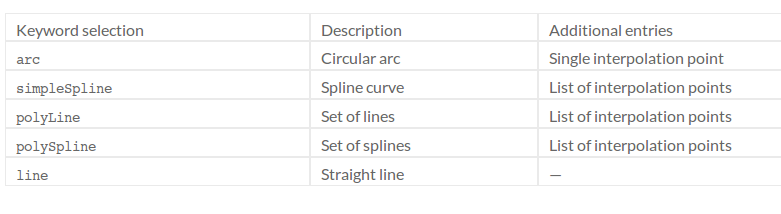
\includegraphics[scale=0.6]{ref.png}
\caption{Types of edges used in BlockMeshDict dictionary}
\label{ref}
\end{center}  
\end{figure}

\flushleft For this problem we have used arc edges. Therfore the details within edges can be given as{$:$}
\flushleft edges
\flushleft (
 \flushleft{$<$}keyword{$>$} {$<$}vertices joining the edge{$>$} (interpolation points)
\flushleft);
\flushleft The details of edges for our current problem is given in fig \ref{edges}{$:$}

\begin{figure}[ht]  
\begin{center}  
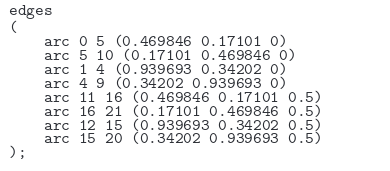
\includegraphics[scale=0.7]{edges.png}
\caption{Edge details for the blockMeshDict file}
\label{edges}
\end{center}  
\end{figure}

\flushleft After this enter the boundary patches under the keyword boundary. You may refer to the previous chapter to get know more details regarding how to write the boundary patches.
\flushleft Similar to the lid-driven cavity problem , even this geometry does not have any patches to be merged. Therefore we will keep the mergePatchPairs empty.
\flushleft After completing the blockMeshDict file, you can save it within the required case file in polymesh folder inside constant folder. Thereafter switch back to the command terminal and open the required case file as mentioned in the previous chapter.
\flushleft After this enter blockMesh in the command terminal and press $<enter>$. Thus you can see geometry is meshed. After this type paraFoam in the command terminal and press{$<$}enter{$>$}. This opens the ParaView window. Now on the ParaView window press apply on the left hand side of the Object Inspector Menu to view the new geometry.

\begin{figure}[ht]  
\begin{center}  
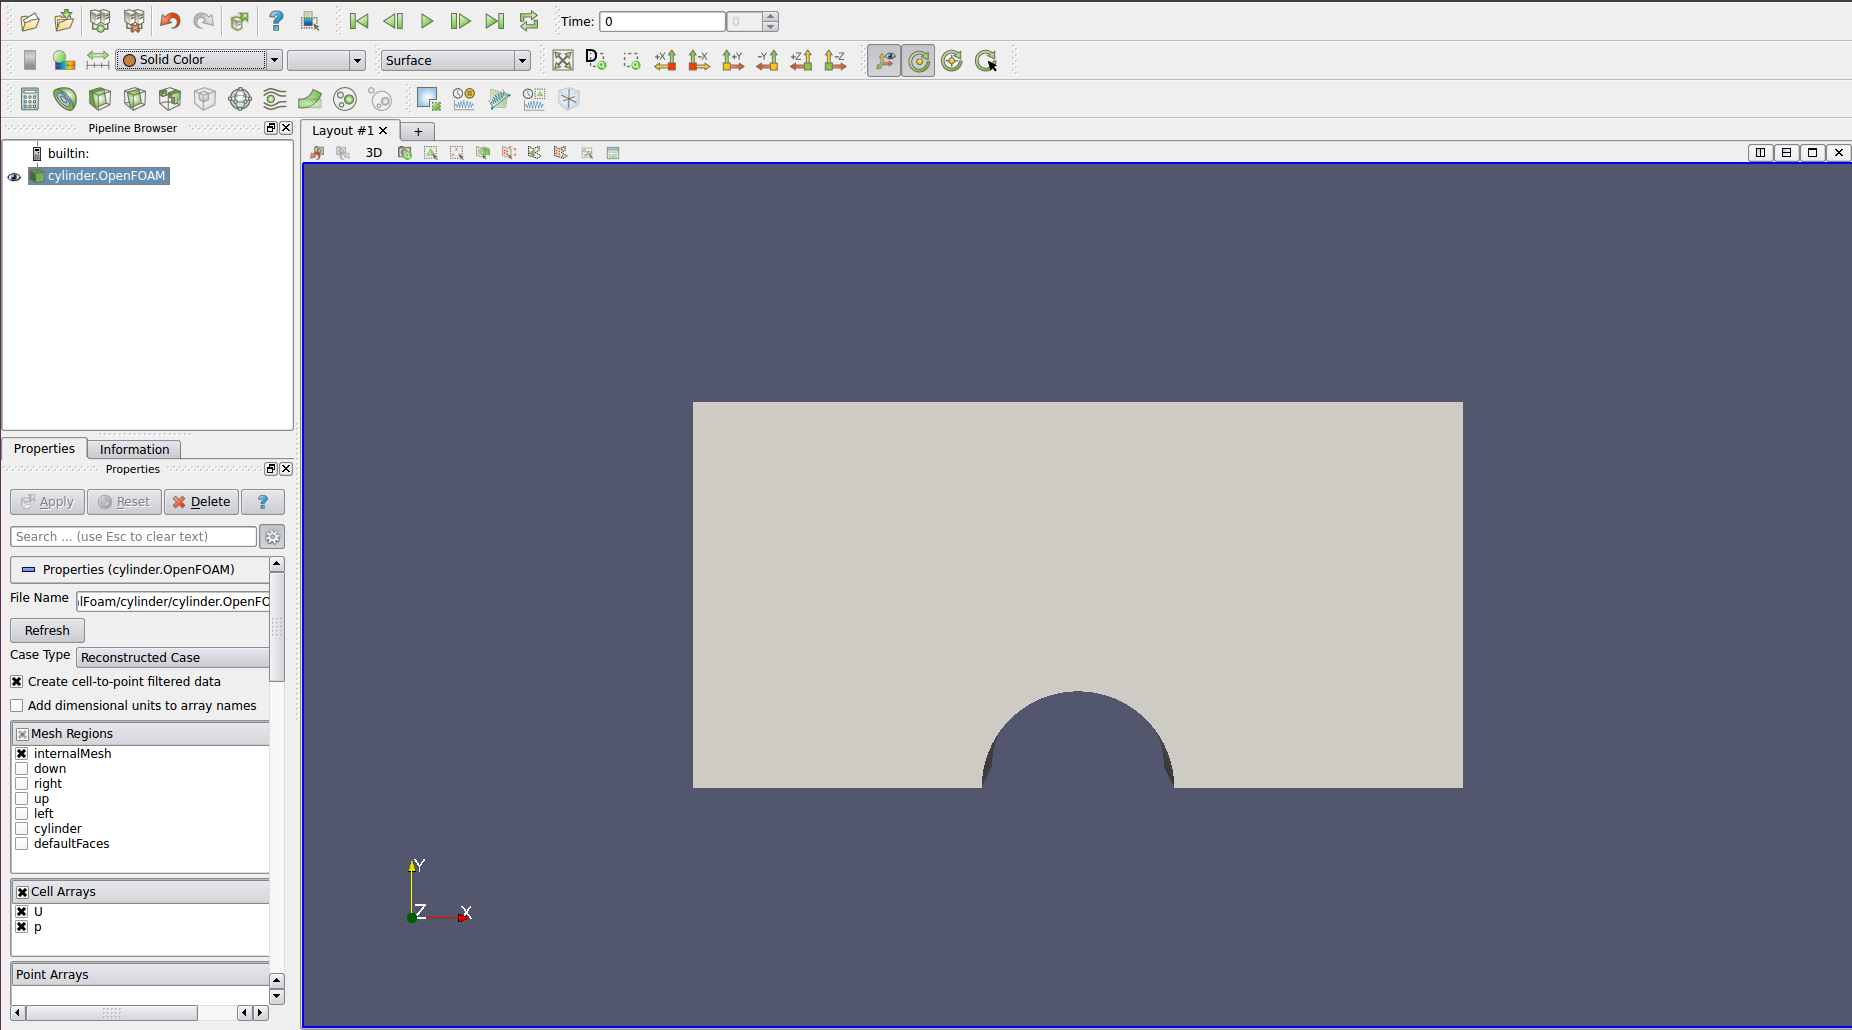
\includegraphics[scale=0.25]{paraview1.png}
\caption{ParaView window showing the 2-D geometry}
\label{paraview1}
\end{center}  
\end{figure}

\flushleft Now in the ParaView window you can check or uncheck the different regions within the mesh region in  the Object Inspector Menu to visualize differnt regions on the geomtery. You can also visualize the geometry in wire-frame instead of surface by changing it from the down-down Active Variable Control Menu.
\flushleft Thus in this chapter we learned how to create a curved geometry in OpenFOAM and visualize it in different ways using ParaView.
\end{document}
